\documentclass[11pt]{article}
\usepackage[textwidth=18.0cm, textheight=23.0cm, top=2.0cm]{geometry}
\usepackage{pst-all}
\usepackage{amssymb}
\usepackage{tikz}
\usepackage{underscore}\begin{document}
\pagestyle{empty}


ClassName: \underline{\textbf{Class_03.2bp-13}}
\par
BinSize: \underline{\textbf{40 × 40}}
\par
ReduceSize: \underline{\textbf{40 × 40}}
\par
TypeNum: \underline{\textbf{40}}
\par
Num: \underline{\textbf{40}}
\par
OutS: \underline{\textbf{16000}}
\par
InS: \underline{\textbf{13176}}
\par
Rate: \underline{\textbf{0.824}}
\par
UB: \underline{\textbf{10}}
\par
LB0: \underline{\textbf{10}}
\par
LB: \underline{\textbf{10}}
\par
LBWithCut: \underline{\textbf{10}}
\par
NodeCut: \underline{\textbf{0}}
\par
ExtendedNodeCnt: \underline{\textbf{1}}
\par
GenNodeCnt: \underline{\textbf{1}}
\par
PrimalNode: \underline{\textbf{0}}
\par
ColumnCount: \underline{\textbf{10}}
\par
TotalCutCount: \underline{\textbf{0}}
\par
RootCutCount: \underline{\textbf{0}}
\par
LPSolverCnt: \underline{\textbf{1}}
\par
PricingSolverCnt: \underline{\textbf{0}}
\par
BranchAndBoundNum: \underline{\textbf{1}}
\par
isOpt: \underline{\textbf{true}}
\par
TimeOnInitSolution: \underline{\textbf{0.020 s}}
\par
TimeOnPrimal: \underline{\textbf{0.000 s}}
\par
TimeOnPricing: \underline{\textbf{0.000 s}}
\par
TimeOnRmp: \underline{\textbf{0.063 s}}
\par
TotalTime: \underline{\textbf{0.145 s}}
\par
\newpage


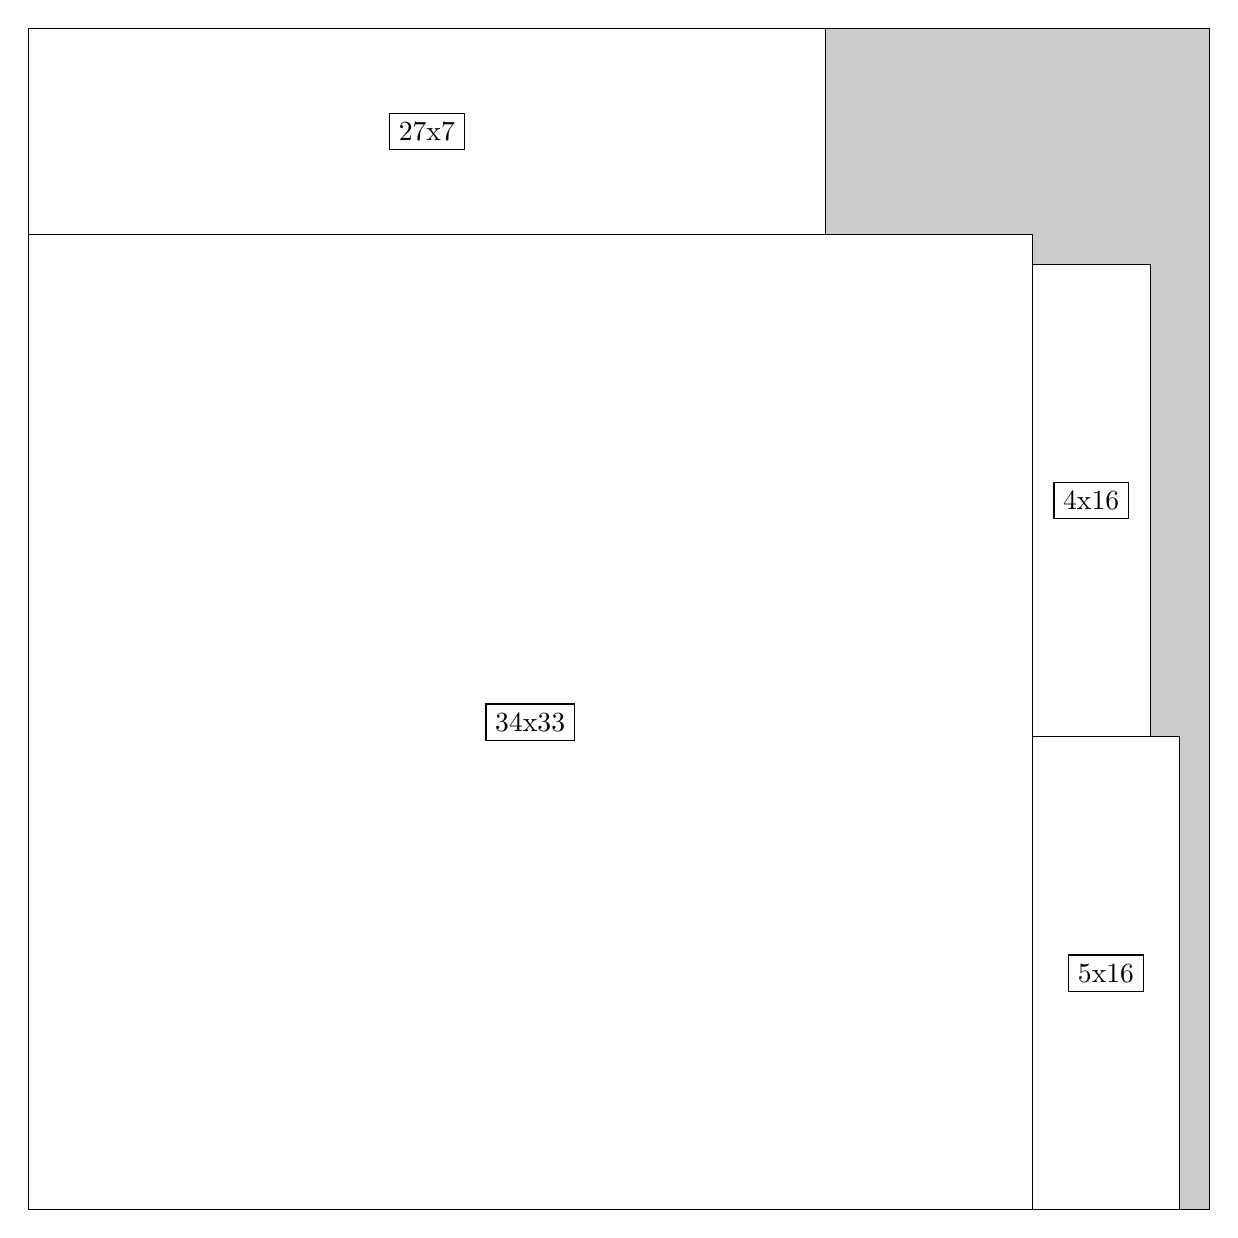
\begin{tikzpicture}[shorten >=1pt,scale=1.0,every node/.style={scale=1.0},->]
\tikzstyle{vertex}=[circle,fill=black!25,minimum size=14pt,inner sep=0pt]
\filldraw[fill=gray!40!white, draw=black] (0,0) rectangle (15.0,15.0);
\foreach \name/\x/\y/\w/\h in {34x33/0.0/0.0/12.75/12.375,27x7/0.0/12.375/10.125/2.625,5x16/12.75/0.0/1.875/6.0,4x16/12.75/6.0/1.5/6.0}
\filldraw[fill=white!40!white, draw=black] (\x,\y) rectangle node[draw] (\name) {\name} ++(\w,\h);
\end{tikzpicture}


w =34 , h =33 , x =0 , y =0 , v =1122
\par
w =27 , h =7 , x =0 , y =33 , v =189
\par
w =5 , h =16 , x =34 , y =0 , v =80
\par
w =4 , h =16 , x =34 , y =16 , v =64
\par
\newpage


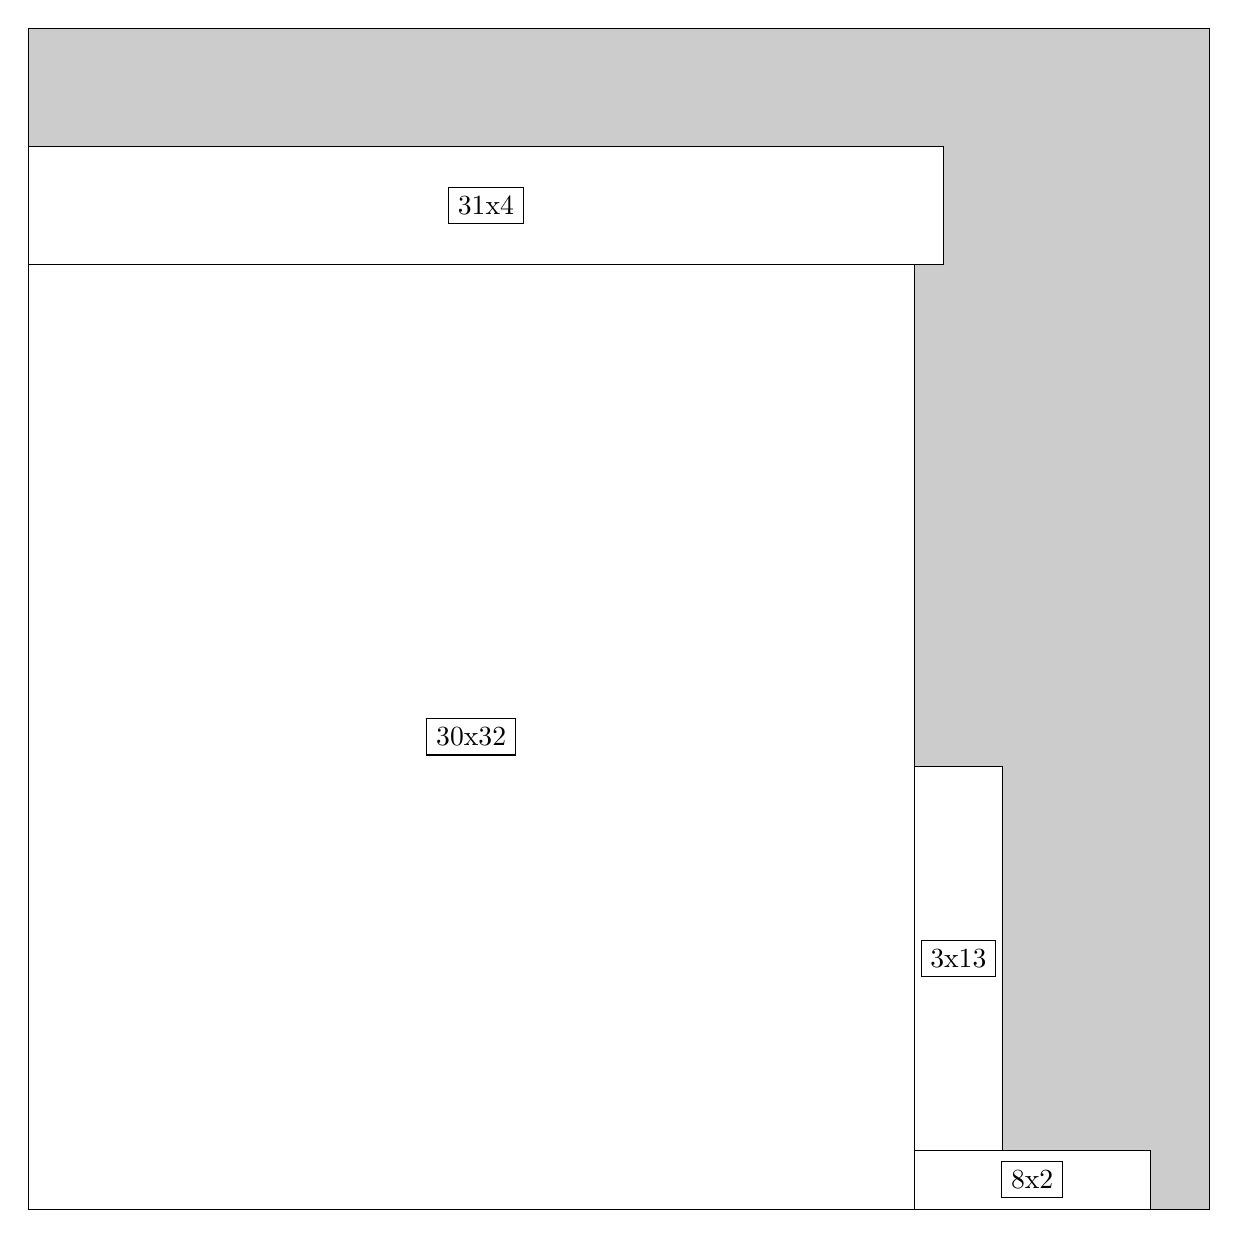
\begin{tikzpicture}[shorten >=1pt,scale=1.0,every node/.style={scale=1.0},->]
\tikzstyle{vertex}=[circle,fill=black!25,minimum size=14pt,inner sep=0pt]
\filldraw[fill=gray!40!white, draw=black] (0,0) rectangle (15.0,15.0);
\foreach \name/\x/\y/\w/\h in {30x32/0.0/0.0/11.25/12.0,31x4/0.0/12.0/11.625/1.5,3x13/11.25/0.75/1.125/4.875,8x2/11.25/0.0/3.0/0.75}
\filldraw[fill=white!40!white, draw=black] (\x,\y) rectangle node[draw] (\name) {\name} ++(\w,\h);
\end{tikzpicture}


w =30 , h =32 , x =0 , y =0 , v =960
\par
w =31 , h =4 , x =0 , y =32 , v =124
\par
w =3 , h =13 , x =30 , y =2 , v =39
\par
w =8 , h =2 , x =30 , y =0 , v =16
\par
\newpage


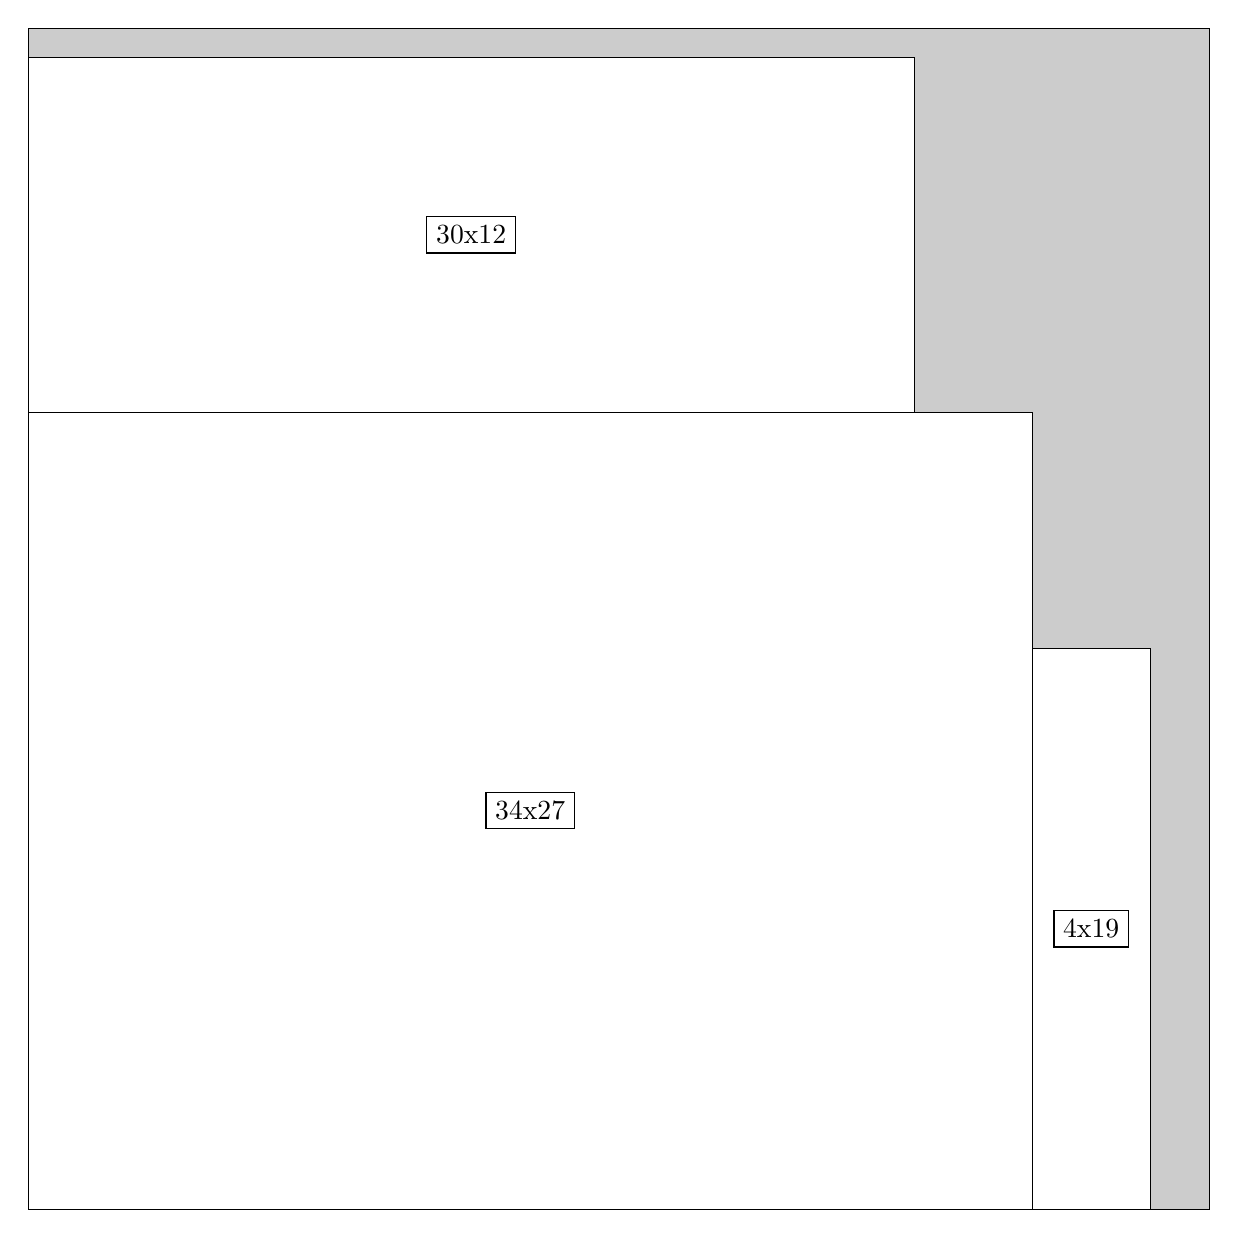
\begin{tikzpicture}[shorten >=1pt,scale=1.0,every node/.style={scale=1.0},->]
\tikzstyle{vertex}=[circle,fill=black!25,minimum size=14pt,inner sep=0pt]
\filldraw[fill=gray!40!white, draw=black] (0,0) rectangle (15.0,15.0);
\foreach \name/\x/\y/\w/\h in {34x27/0.0/0.0/12.75/10.125,30x12/0.0/10.125/11.25/4.5,4x19/12.75/0.0/1.5/7.125}
\filldraw[fill=white!40!white, draw=black] (\x,\y) rectangle node[draw] (\name) {\name} ++(\w,\h);
\end{tikzpicture}


w =34 , h =27 , x =0 , y =0 , v =918
\par
w =30 , h =12 , x =0 , y =27 , v =360
\par
w =4 , h =19 , x =34 , y =0 , v =76
\par
\newpage


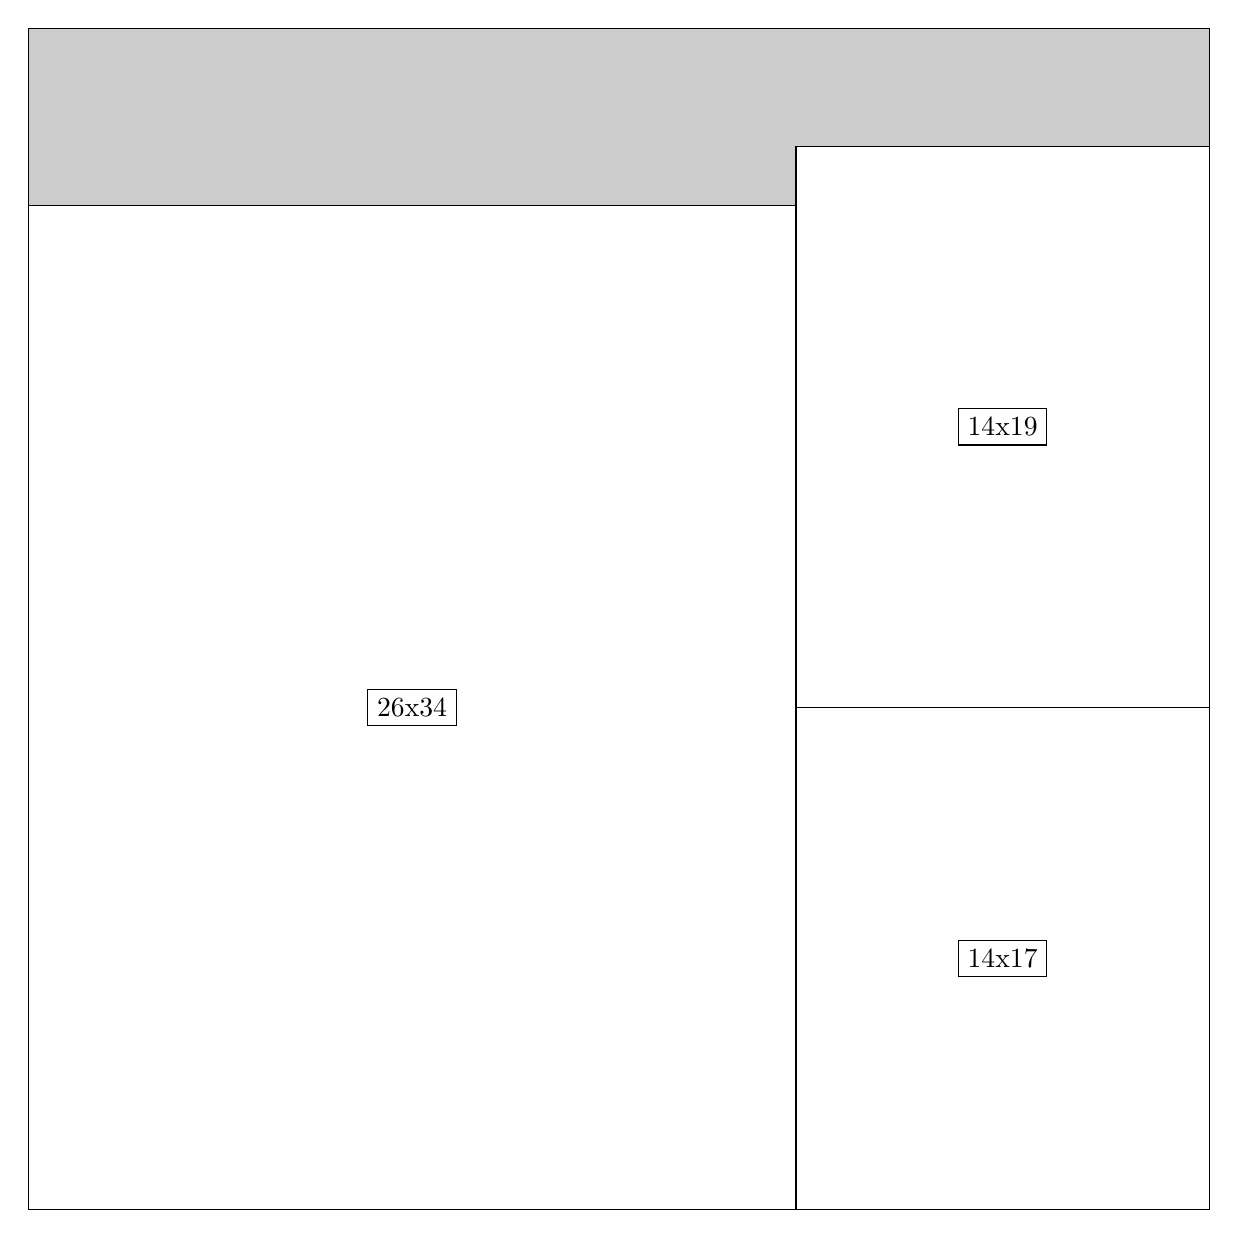
\begin{tikzpicture}[shorten >=1pt,scale=1.0,every node/.style={scale=1.0},->]
\tikzstyle{vertex}=[circle,fill=black!25,minimum size=14pt,inner sep=0pt]
\filldraw[fill=gray!40!white, draw=black] (0,0) rectangle (15.0,15.0);
\foreach \name/\x/\y/\w/\h in {26x34/0.0/0.0/9.75/12.75,14x19/9.75/6.375/5.25/7.125,14x17/9.75/0.0/5.25/6.375}
\filldraw[fill=white!40!white, draw=black] (\x,\y) rectangle node[draw] (\name) {\name} ++(\w,\h);
\end{tikzpicture}


w =26 , h =34 , x =0 , y =0 , v =884
\par
w =14 , h =19 , x =26 , y =17 , v =266
\par
w =14 , h =17 , x =26 , y =0 , v =238
\par
\newpage


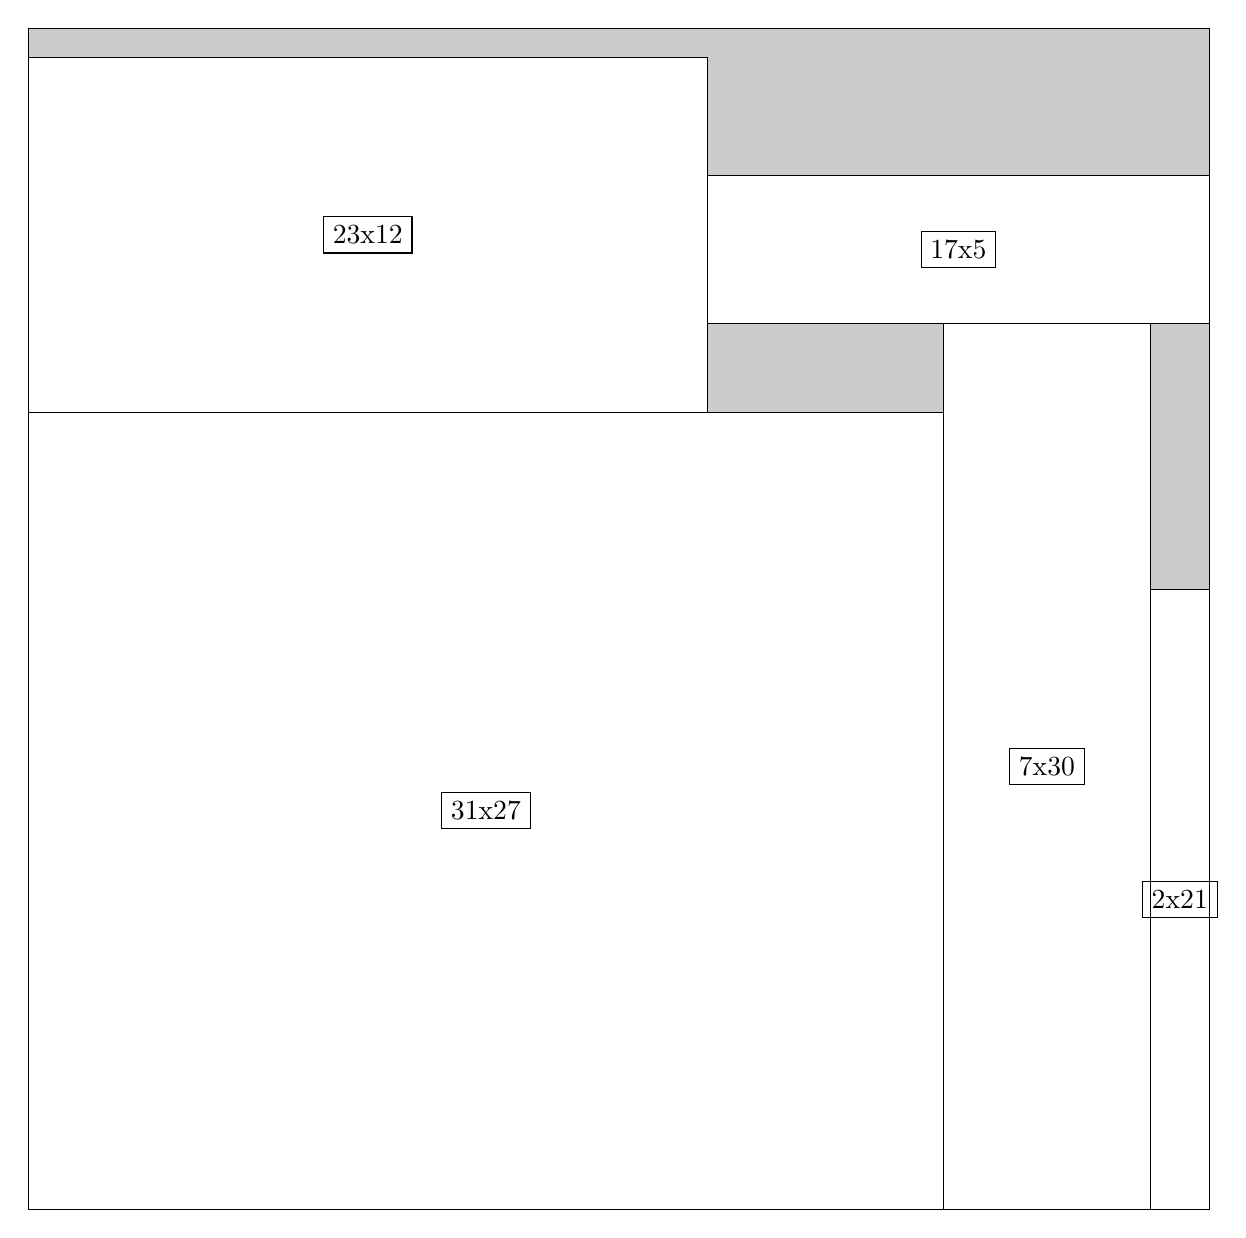
\begin{tikzpicture}[shorten >=1pt,scale=1.0,every node/.style={scale=1.0},->]
\tikzstyle{vertex}=[circle,fill=black!25,minimum size=14pt,inner sep=0pt]
\filldraw[fill=gray!40!white, draw=black] (0,0) rectangle (15.0,15.0);
\foreach \name/\x/\y/\w/\h in {31x27/0.0/0.0/11.625/10.125,7x30/11.625/0.0/2.625/11.25,23x12/0.0/10.125/8.625/4.5,17x5/8.625/11.25/6.375/1.875,2x21/14.25/0.0/0.75/7.875}
\filldraw[fill=white!40!white, draw=black] (\x,\y) rectangle node[draw] (\name) {\name} ++(\w,\h);
\end{tikzpicture}


w =31 , h =27 , x =0 , y =0 , v =837
\par
w =7 , h =30 , x =31 , y =0 , v =210
\par
w =23 , h =12 , x =0 , y =27 , v =276
\par
w =17 , h =5 , x =23 , y =30 , v =85
\par
w =2 , h =21 , x =38 , y =0 , v =42
\par
\newpage


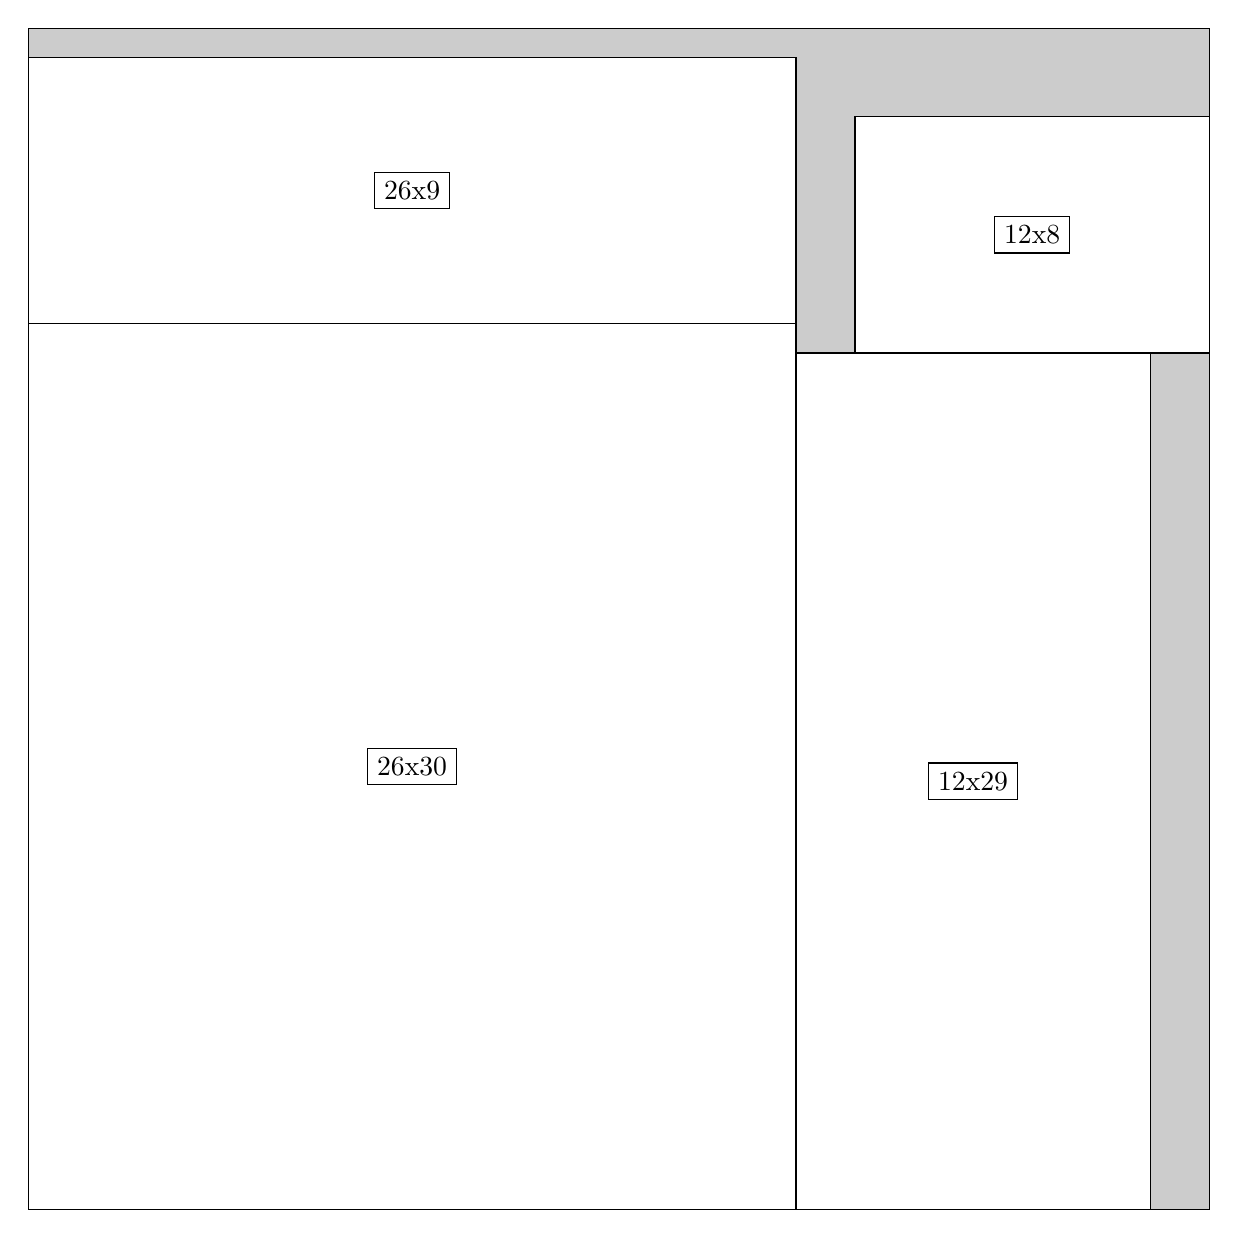
\begin{tikzpicture}[shorten >=1pt,scale=1.0,every node/.style={scale=1.0},->]
\tikzstyle{vertex}=[circle,fill=black!25,minimum size=14pt,inner sep=0pt]
\filldraw[fill=gray!40!white, draw=black] (0,0) rectangle (15.0,15.0);
\foreach \name/\x/\y/\w/\h in {26x30/0.0/0.0/9.75/11.25,12x29/9.75/0.0/4.5/10.875,26x9/0.0/11.25/9.75/3.375,12x8/10.5/10.875/4.5/3.0}
\filldraw[fill=white!40!white, draw=black] (\x,\y) rectangle node[draw] (\name) {\name} ++(\w,\h);
\end{tikzpicture}


w =26 , h =30 , x =0 , y =0 , v =780
\par
w =12 , h =29 , x =26 , y =0 , v =348
\par
w =26 , h =9 , x =0 , y =30 , v =234
\par
w =12 , h =8 , x =28 , y =29 , v =96
\par
\newpage


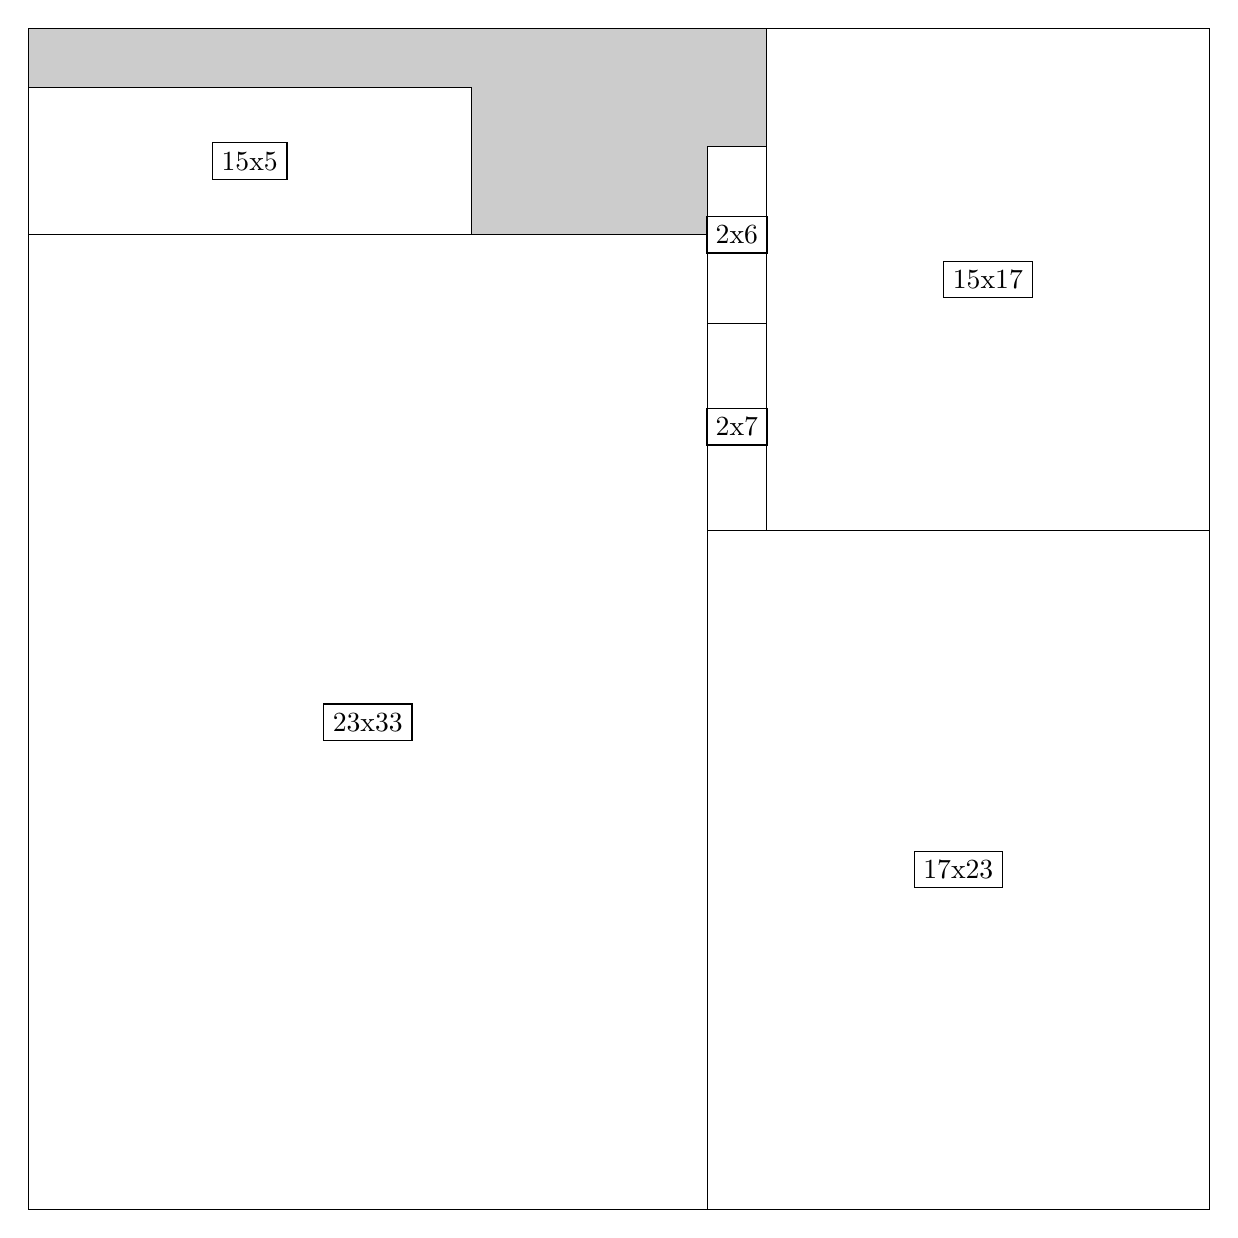
\begin{tikzpicture}[shorten >=1pt,scale=1.0,every node/.style={scale=1.0},->]
\tikzstyle{vertex}=[circle,fill=black!25,minimum size=14pt,inner sep=0pt]
\filldraw[fill=gray!40!white, draw=black] (0,0) rectangle (15.0,15.0);
\foreach \name/\x/\y/\w/\h in {23x33/0.0/0.0/8.625/12.375,17x23/8.625/0.0/6.375/8.625,15x17/9.375/8.625/5.625/6.375,15x5/0.0/12.375/5.625/1.875,2x7/8.625/8.625/0.75/2.625,2x6/8.625/11.25/0.75/2.25}
\filldraw[fill=white!40!white, draw=black] (\x,\y) rectangle node[draw] (\name) {\name} ++(\w,\h);
\end{tikzpicture}


w =23 , h =33 , x =0 , y =0 , v =759
\par
w =17 , h =23 , x =23 , y =0 , v =391
\par
w =15 , h =17 , x =25 , y =23 , v =255
\par
w =15 , h =5 , x =0 , y =33 , v =75
\par
w =2 , h =7 , x =23 , y =23 , v =14
\par
w =2 , h =6 , x =23 , y =30 , v =12
\par
\newpage


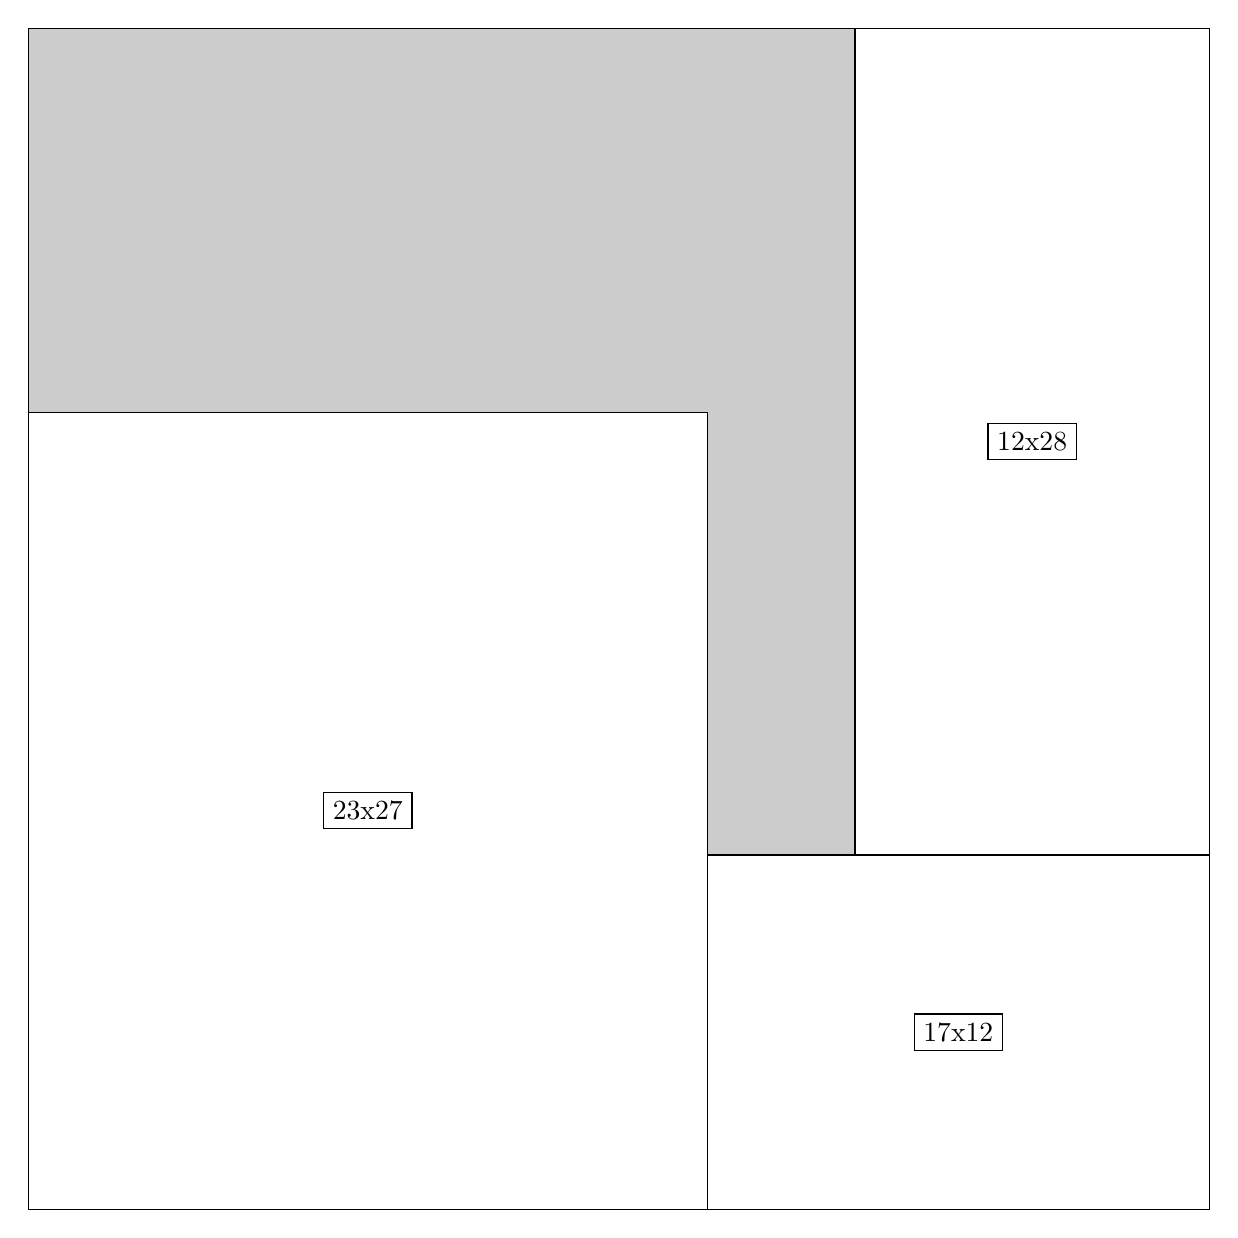
\begin{tikzpicture}[shorten >=1pt,scale=1.0,every node/.style={scale=1.0},->]
\tikzstyle{vertex}=[circle,fill=black!25,minimum size=14pt,inner sep=0pt]
\filldraw[fill=gray!40!white, draw=black] (0,0) rectangle (15.0,15.0);
\foreach \name/\x/\y/\w/\h in {23x27/0.0/0.0/8.625/10.125,12x28/10.5/4.5/4.5/10.5,17x12/8.625/0.0/6.375/4.5}
\filldraw[fill=white!40!white, draw=black] (\x,\y) rectangle node[draw] (\name) {\name} ++(\w,\h);
\end{tikzpicture}


w =23 , h =27 , x =0 , y =0 , v =621
\par
w =12 , h =28 , x =28 , y =12 , v =336
\par
w =17 , h =12 , x =23 , y =0 , v =204
\par
\newpage


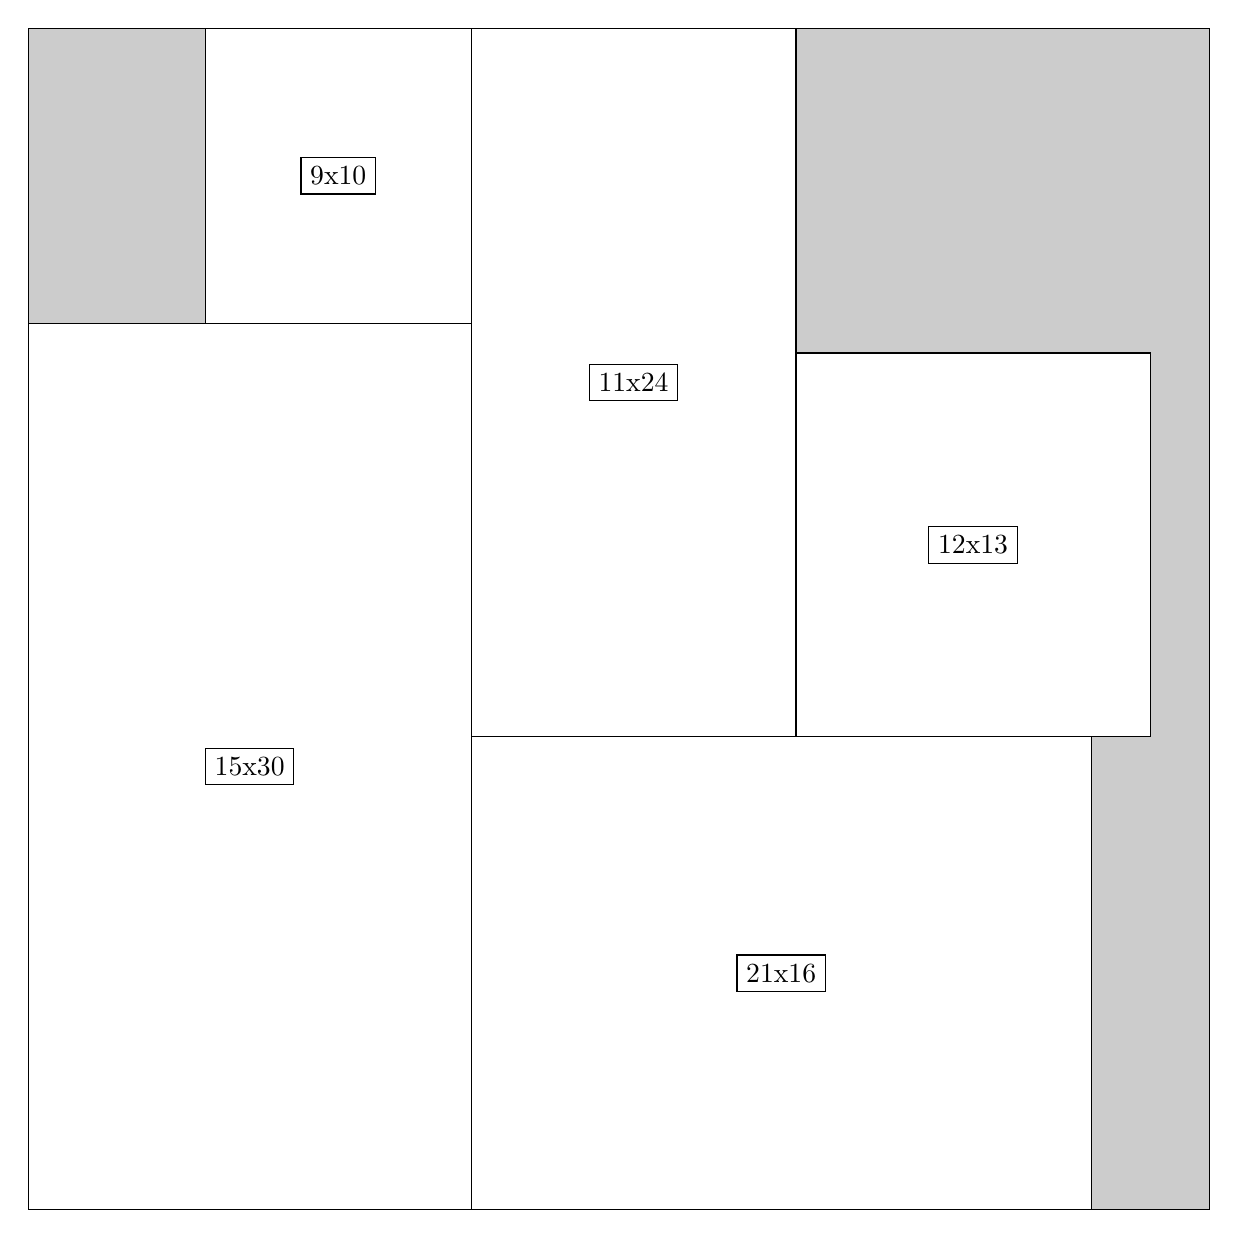
\begin{tikzpicture}[shorten >=1pt,scale=1.0,every node/.style={scale=1.0},->]
\tikzstyle{vertex}=[circle,fill=black!25,minimum size=14pt,inner sep=0pt]
\filldraw[fill=gray!40!white, draw=black] (0,0) rectangle (15.0,15.0);
\foreach \name/\x/\y/\w/\h in {15x30/0.0/0.0/5.625/11.25,21x16/5.625/0.0/7.875/6.0,11x24/5.625/6.0/4.125/9.0,12x13/9.75/6.0/4.5/4.875,9x10/2.25/11.25/3.375/3.75}
\filldraw[fill=white!40!white, draw=black] (\x,\y) rectangle node[draw] (\name) {\name} ++(\w,\h);
\end{tikzpicture}


w =15 , h =30 , x =0 , y =0 , v =450
\par
w =21 , h =16 , x =15 , y =0 , v =336
\par
w =11 , h =24 , x =15 , y =16 , v =264
\par
w =12 , h =13 , x =26 , y =16 , v =156
\par
w =9 , h =10 , x =6 , y =30 , v =90
\par
\newpage


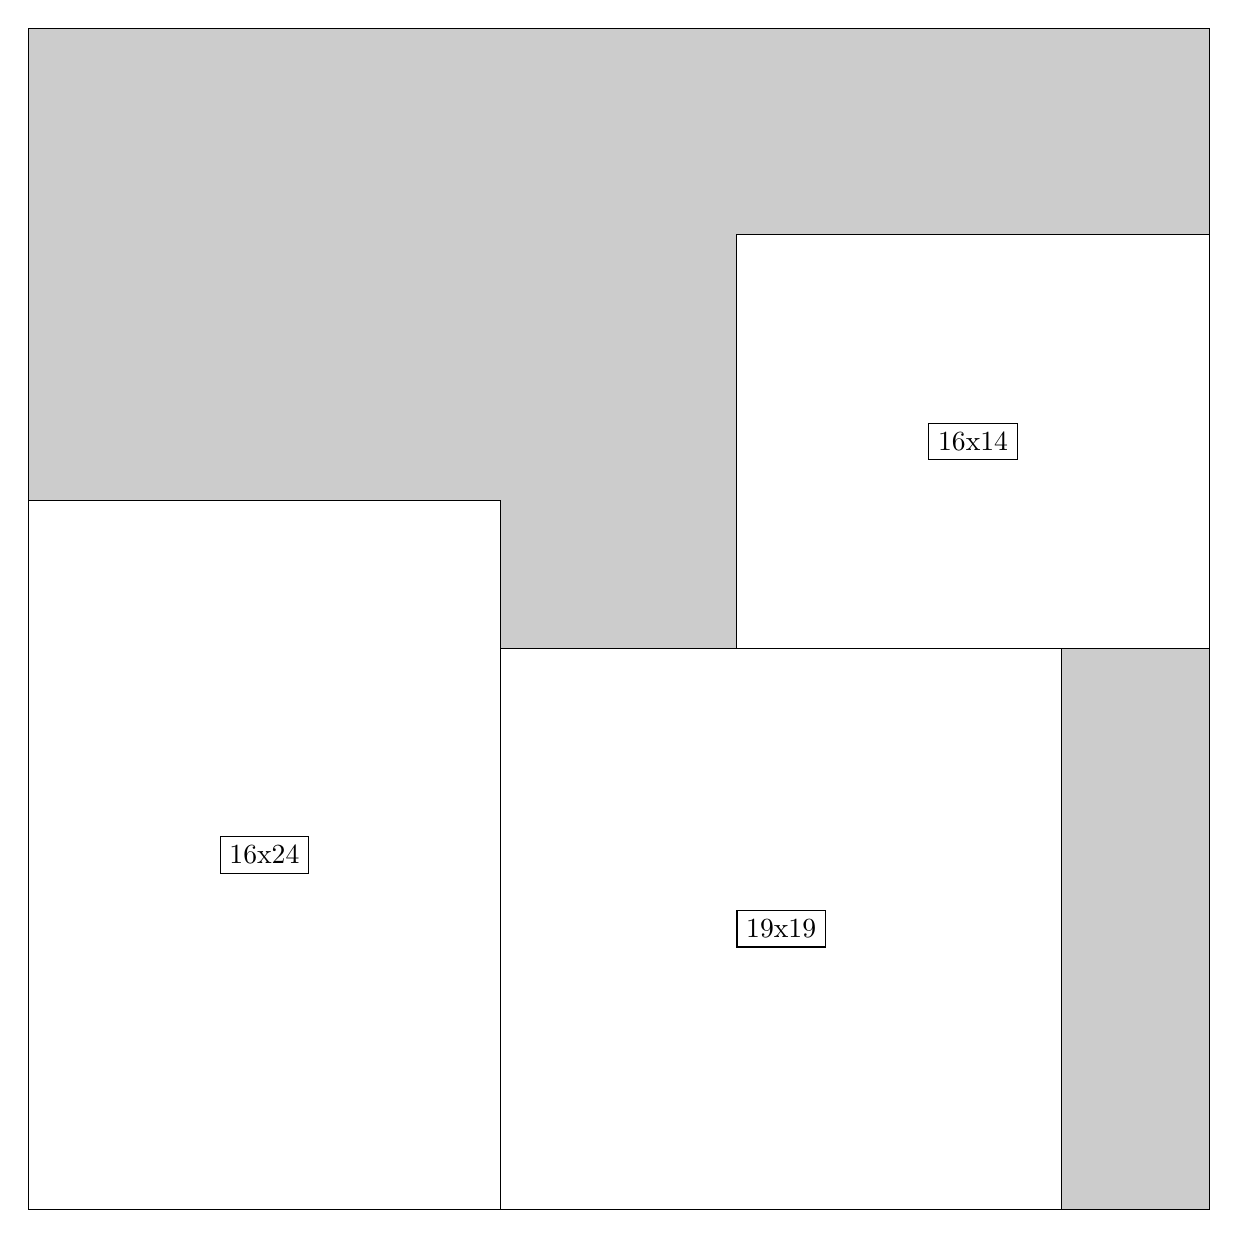
\begin{tikzpicture}[shorten >=1pt,scale=1.0,every node/.style={scale=1.0},->]
\tikzstyle{vertex}=[circle,fill=black!25,minimum size=14pt,inner sep=0pt]
\filldraw[fill=gray!40!white, draw=black] (0,0) rectangle (15.0,15.0);
\foreach \name/\x/\y/\w/\h in {16x24/0.0/0.0/6.0/9.0,19x19/6.0/0.0/7.125/7.125,16x14/9.0/7.125/6.0/5.25}
\filldraw[fill=white!40!white, draw=black] (\x,\y) rectangle node[draw] (\name) {\name} ++(\w,\h);
\end{tikzpicture}


w =16 , h =24 , x =0 , y =0 , v =384
\par
w =19 , h =19 , x =16 , y =0 , v =361
\par
w =16 , h =14 , x =24 , y =19 , v =224
\par
\newpage


\end{document}